\documentclass[12pt,a4paper]{article}

\usepackage[T1]{fontenc}
\usepackage[polish]{babel}
\usepackage[utf8]{inputenc}
\usepackage{lmodern}
\selectlanguage{polish}
\usepackage{graphicx}
\usepackage{cite}
\usepackage{csquotes}
\usepackage{hyperref}
\usepackage{float}
\usepackage{amsmath}
\usepackage{tabularx}
\usepackage{array}
\usepackage{booktabs}
\usepackage{geometry}
\usepackage{enumitem}
\usepackage{xcolor}

\geometry{margin=2.5cm}

\definecolor{gmail}{HTML}{FF6A3D}
\definecolor{outlook}{HTML}{0D8F8D}

\begin{document}

%% --- STRONA TYTUŁOWA ---
\pagenumbering{gobble}
\clearpage
\begin{figure}[H]
\centering
\includegraphics[width=0.4\textwidth]{media/ps-logo.png}
\end{figure}

\vspace{1cm}
\begin{center}
    \Large\textbf{Projekt Seminarium}
\end{center}
\vspace{0.5cm}
\begin{center}
    \Large\textbf{Badanie porównawcze interakcji użytkownika na platformach pocztowych: Gmail vs Outlook}
\end{center}

\vspace{2cm}
\begin{center}\large\textbf{Marcin i Jan}\end{center}
\vspace{1.5cm}

\begin{center}\large\textbf{Kierunek: Informatyka (profil praktyczny)}\end{center}
\begin{center}\large\textbf{Specjalność: Uczenie Maszynowe}\end{center}
\vspace{2cm}
\begin{center}\large\textbf{Gliwice 2026}\end{center}

%% --- SPIS TREŚCI ---
\newpage
\pagenumbering{arabic}
\tableofcontents
\newpage

%% === 1. OKREŚLENIE WZORCOWYCH ELEMENTÓW INTERAKCJI ===
\section{Określenie wzorcowych elementów interakcji dla badanej klasy rozwiązań/aplikacji}

\subsection{Charakterystyka badanej klasy}

Badana klasa obejmuje \textbf{webowe klienty pocztowe} --- aplikacje umożliwiające zarządzanie korespondencją elektroniczną poprzez przeglądarkę internetową. Kluczowe elementy interakcji w tej klasie to:

\begin{itemize}[noitemsep]
    \item \textbf{Nawigacja} --- struktura widoków, hierarchia folderów/etykiet, czytelność menu
    \item \textbf{Zarządzanie treścią} --- tworzenie, edycja, usuwanie wiadomości
    \item \textbf{Wyszukiwanie} --- lokalizacja konkretnych wiadomości wśród large zbiorów
    \item \textbf{Organizacja} --- etykiety, foldery, archiwizacja, masowe operacje
    \item \textbf{Informacja zwrotna} --- komunikaty o stanie akcji (wysłano, zapisano, błąd)
    \item \textbf{Wydajność} --- czas odpowiedzi interfejsu na akcje użytkownika
\end{itemize}

\subsection{Zdefiniowane kryteria oceny}

Na podstawie analizy literatury z zakresu UX (Nielsen, Tognazzini) oraz specyfiki klientów pocztowych zdefiniowano \textbf{8 kryteriów oceny}:

\begin{table}[H]
\centering
\caption{Kryteria oceny interfejsu klienta pocztowego}
\label{tab:kryteria}
\begin{tabularx}{\textwidth}{|c|X|X|}
\hline
\textbf{Nr} & \textbf{Kryterium} & \textbf{Opis} \\
\hline
Q1 & Łatwość rozpoczęcia pracy & Jak szybko i intuicyjnie da się rozpocząć realizację zadania po wejściu do interfejsu \\
\hline
Q2 & Czytelność nawigacji i układu & Czy struktura widoków, etykiety i rozmieszczenie elementów prowadzą użytkownika bez zgadywania \\
\hline
Q3 & Wyszukiwanie i filtrowanie wiadomości & Precyzja wyników, łatwość użycia filtrów oraz czas dojścia do właściwej wiadomości \\
\hline
Q4 & Tworzenie i edycja wiadomości & Komfort pisania, formatowania, dodawania odbiorców i załączników oraz poprawiania treści \\
\hline
Q5 & Zarządzanie skrzynką & Działania na wiadomościach: oznaczanie, przenoszenie, archiwizacja, etykiety/foldery, masowe operacje \\
\hline
Q6 & Widoczność statusu i informacji zwrotnej & Czy system jasno komunikuje wynik akcji: wysłano, zapisano, błąd, synchronizacja itp. \\
\hline
Q7 & Wydajność i szybkość interakcji & Responsywność interfejsu i płynność podczas realizacji typowych zadań \\
\hline
Q8 & Ogólna satysfakcja z doświadczenia & Całościowe odczucie pracy z platformą po wykonaniu wszystkich zadań testowych \\
\hline
\end{tabularx}
\end{table}

\subsection{Schemat pomiaru}

Każde kryterium oceniane jest \textbf{niezależnie dla każdej platformy} (Gmail i Outlook) w skali 1--10, gdzie:
\begin{itemize}[noitemsep]
    \item \textbf{1} --- bardzo słabo
    \item \textbf{5} --- neutralnie
    \item \textbf{10} --- bardzo dobrze
\end{itemize}

Dodatkowo respondent wskazuje \textbf{ogólną preferencję} (Gmail / Outlook / Remis) oraz podaje swój \textbf{wiek}.

%% === 2. PRZEGLĄD POTENCJALNYCH ROZWIĄZAŃ ===
\newpage
\section{Przegląd potencjalnych rozwiązań --- kandydatów do ewaluacji}

\subsection{Wybrane platformy}

Do badania wybrano dwie wiodące platformy pocztowe:

\begin{table}[H]
\centering
\caption{Porównanie wybranych platform pocztowych}
\label{tab:platformy}
\begin{tabularx}{\textwidth}{|X|X|X|}
\hline
\textbf{Cecha} & \textbf{Gmail (Google Workspace)} & \textbf{Outlook (Microsoft 365)} \\
\hline
Rynek & Dominujący na rynku konsumenckim & Popularny w środowisku korporacyjnym \\
\hline
Interfejs webowy & Material Design, minimalistyczny & Fluent UI, zintegrowany z pakietem Office \\
\hline
Darmowa wersja & Tak (15 GB) & Tak (15 GB) \\
\hline
Integracje & Google Drive, Kalendarz, Meet & OneDrive, Kalendarz, Teams \\
\hline
Mobilność & Aplikacja Gmail (iOS/Android) & Aplikacja Outlook (iOS/Android) \\
\hline
\end{tabularx}
\end{table}

\subsection{Kryteria wyboru}

Platformy wybrano na podstawie:
\begin{enumerate}[noitemsep]
    \item \textbf{Popularności} --- obie mają setki milionów użytkowników na świecie
    \item \textbf{Dostępności webowej} --- obie oferują pełną funkcjonalność w przeglądarce
    \item \textbf{Różnorodności podejść} --- Gmail (Google, Material Design) vs Outlook (Microsoft, Fluent UI) reprezentują odmienne filozofie projektowania interfejsów
    \item \textbf{Dostępności} --- minimalne wymagania sprzętowe, brak konieczności instalacji
\end{enumerate}

\subsection{Ograniczenia wyboru}

\begin{itemize}[noitemsep]
    \item Nie uwzględniono klientów desktopowych (Thunderbird, Apple Mail)
    \item Nie porównywano wersji mobilnych
    \item Nie badano integracji z zewnętrznymi narzędziami (CRM, task management)
\end{itemize}

%% === 3. OPRACOWANIE SCHEMATU/METODOLOGII BADAŃ ===
\newpage
\section{Opracowanie schematu/metodologii badań}

\subsection{Sposób pomiaru}

\begin{table}[H]
\centering
\caption{Elementy pomiaru w badaniu}
\label{tab:pomiar}
\begin{tabularx}{\textwidth}{|X|X|X|}
\hline
\textbf{Element pomiaru} & \textbf{Format} & \textbf{Opis} \\
\hline
Ocena kryteriów & Skala 1--10 (Gmail + Outlook) & 8 kryteriów $\times$ 2 platformy = 16 ocen na respondenta \\
\hline
Preferencja końcowa & Wybór: Gmail / Outlook / Remis & Po wykonaniu wszystkich zadań \\
\hline
Wiek respondenta & Liczba całkowita (10--100) & Do analizy wg grup wiekowych \\
\hline
Pseudonim & Tekst (opcjonalny) & Identyfikacja respondenta \\
\hline
Komentarz & Tekst (opcjonalny) & Uwagi i spostrzeżenia \\
\hline
\end{tabularx}
\end{table}

\subsection{Grupy wiekowe}

Badanie uwzględnia podział na 4 grupy wiekowe:

\begin{table}[H]
\centering
\caption{Grupy wiekowe respondentów}
\label{tab:grupy_wiekowe}
\begin{tabular}{|l|c|c|}
\hline
\textbf{Grupa} & \textbf{Zakres} & \textbf{Liczba respondentów} \\
\hline
Młodzi & 15--25 & 14 \\
\hline
Średniozaawansowani & 26--35 & 2 \\
\hline
Dojrzali & 36--44 & 1 \\
\hline
Doświadczeni & 45--60 & 1 \\
\hline
\end{tabular}
\end{table}

\subsection{Narzędzia}

\begin{enumerate}[noitemsep]
    \item \textbf{Aplikacja webowa} (HTML/CSS/JS)
    \begin{itemize}[noitemsep]
        \item Formularz ankiety z dynamiczną skalą punktową
        \item Zapis danych do bazy \textbf{Supabase} (PostgreSQL) via REST API
        \item Row Level Security (RLS): anonimowy zapis i odczyt
        \item Informacja o konieczności zwracania uwagi na czas wykonania zadania
    \end{itemize}

    \item \textbf{Panel analizy} (Chart.js)
    \begin{itemize}[noitemsep]
        \item Wykresy porównawcze w czasie rzeczywistym
        \item Analiza wg grup wiekowych
        \item Kompletność odpowiedzi
    \end{itemize}

    \item \textbf{Skrypt generujący wykresy} (Python / matplotlib)
    \begin{itemize}[noitemsep]
        \item Eksport PNG do folderu \texttt{charts/}
        \item Automatyczne pobieranie danych z Supabase
    \end{itemize}
\end{enumerate}

\subsection{Przebieg badania}

\begin{enumerate}[noitemsep]
    \item Uczestnik otwiera ankietę pod adresem URL aplikacji
    \item Zapoznaje się z informacją o zwracaniu uwagi na czas wykonania zadania
    \item Podaje wiek (wymagany) i opcjonalnie pseudonim
    \item Na obu platformach (Gmail i Outlook) wykonuje zestaw typowych zadań:
    \begin{itemize}[noitemsep]
        \item Wyszukanie konkretnej wiadomości
        \item Utworzenie nowej wiadomości z załącznikiem
        \item Oznaczenie/przeniesienie wiadomości
        \item Sprawdzenie statusu wysyłki
    \end{itemize}
    \item Po zakończeniu zadań na obu platformach wypełnia ankietę, oceniając każde kryterium
    \item Na końcu wskazuje ogólną preferencję platformy
    \item Klika ``Zapisz odpowiedzi'' --- dane trafiają do bazy
\end{enumerate}

\subsection{Liczba prób i testerów}

\begin{table}[H]
\centering
\caption{Parametry badania}
\label{tab:parametry}
\begin{tabular}{|l|l|}
\hline
\textbf{Parametr} & \textbf{Wartość} \\
\hline
Liczba kryteriów & 8 ($\times$2 platformy = 16 ocen) \\
\hline
Liczba respondentów & 18 \\
\hline
Rozkład kompletności & 12 pełnych, 2 w połowie, 4 częściowe \\
\hline
Liczba prób na respondenta & 1 pełna ankieta (lub częściowa) \\
\hline
Grupa wiekowa dominująca & 15--25 lat (78\% respondentów) \\
\hline
\end{tabular}
\end{table}

\subsection{Kompletność danych}

\begin{table}[H]
\centering
\caption{Kompletność odpowiedzi}
\label{tab:kompletnosc}
\begin{tabular}{|l|c|l|}
\hline
\textbf{Kategoria} & \textbf{Liczba} & \textbf{Opis} \\
\hline
Pełne (8 pytań) & 12 & Respondent ocenił wszystkie kryteria \\
\hline
Połowa (4--7 pytań) & 2 & Częściowa ocena \\
\hline
Częściowe (1--3 pytania) & 4 & Minimalna liczba ocen \\
\hline
\end{tabular}
\end{table}

%% === WYKRESY ===
\newpage
\section{Wizualizacja i analiza wyników}

\subsection{Porównanie średnich ocen}

Rysunek~\ref{fig:comparison} przedstawia zbiorcze porównanie średnich ocen Gmail i Outlook dla wszystkich 8 kryteriów. Gmail uzyskuje wyższe średnie w 7 z 8 kryteriów.

\begin{figure}[H]
    \centering
    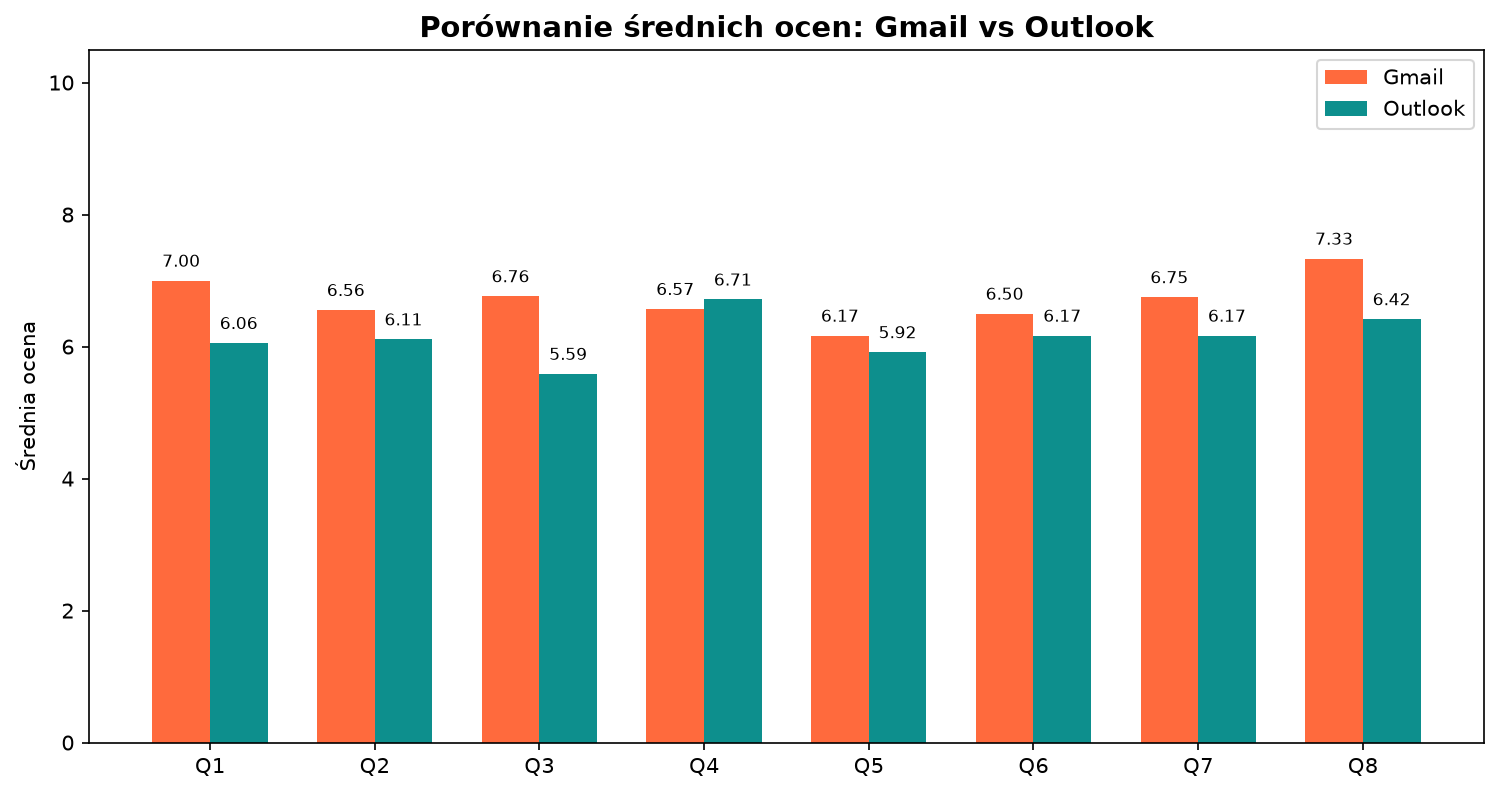
\includegraphics[width=\textwidth]{charts/01_comparison.png}
    \caption{Porównanie średnich ocen: Gmail vs Outlook}
    \label{fig:comparison}
\end{figure}

\subsection{Średnie ocen per pytanie}

Rysunek~\ref{fig:per_question} prezentuje szczegółowe porównanie średnich ocen dla każdego kryterium osobno.

\begin{figure}[H]
    \centering
    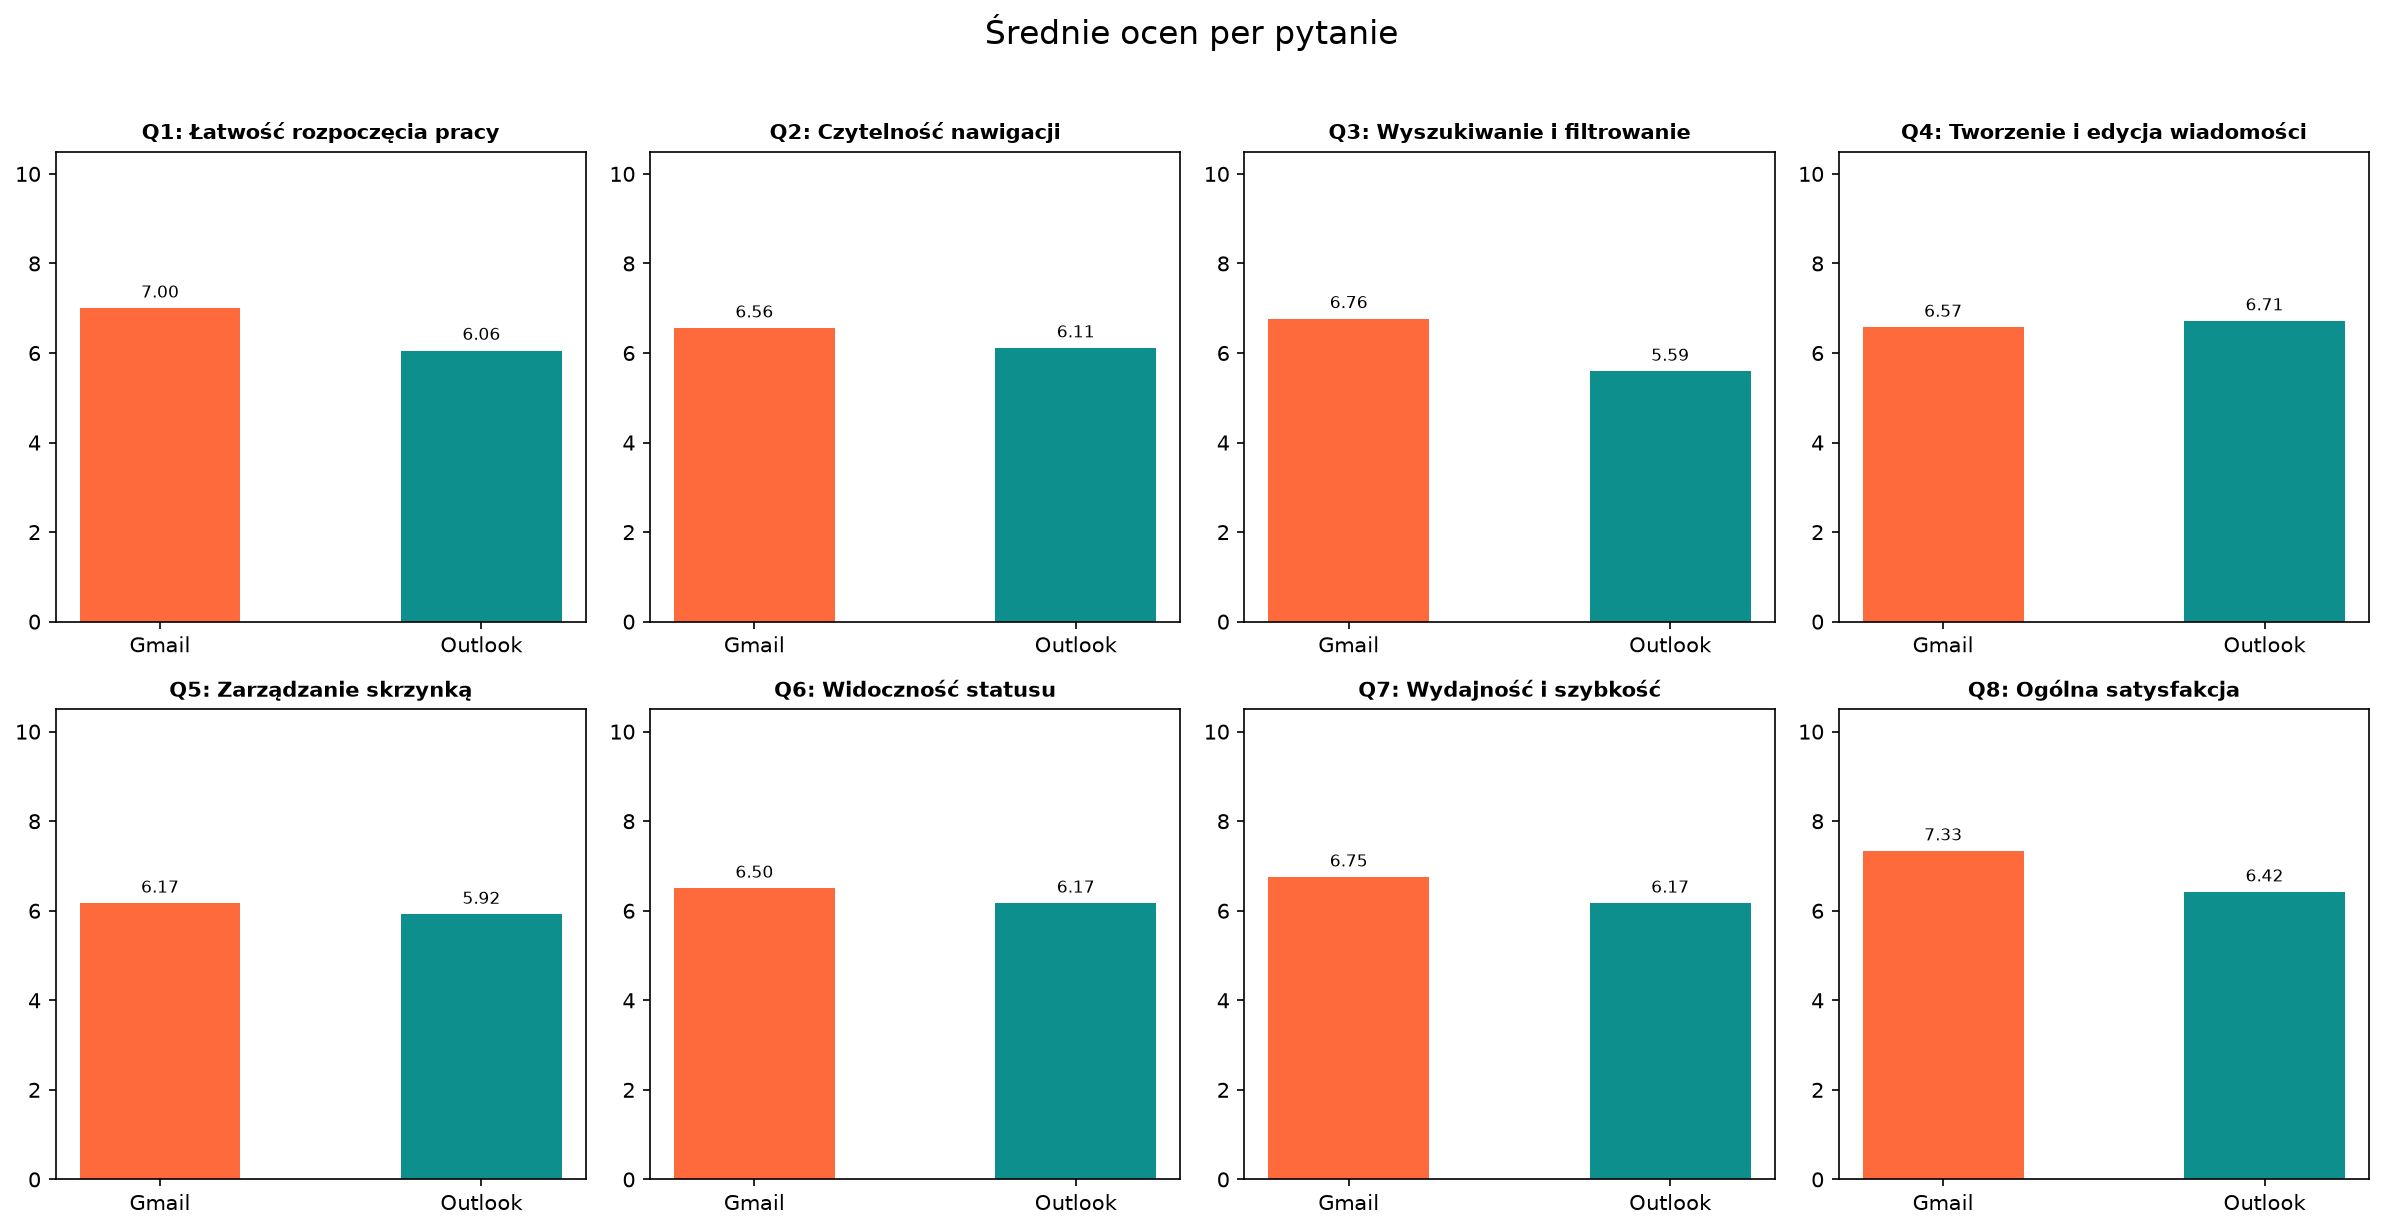
\includegraphics[width=\textwidth]{charts/02_per_question.png}
    \caption{Średnie ocen Gmail vs Outlook dla każdego kryterium}
    \label{fig:per_question}
\end{figure}

\subsection{Preferencja końcowa}

Rysunek~\ref{fig:preference} pokazuje rozkład preferencji końcowych respondentów. Dwie trzecie badanych wskazuje Gmail jako lepszą platformę.

\begin{figure}[H]
    \centering
    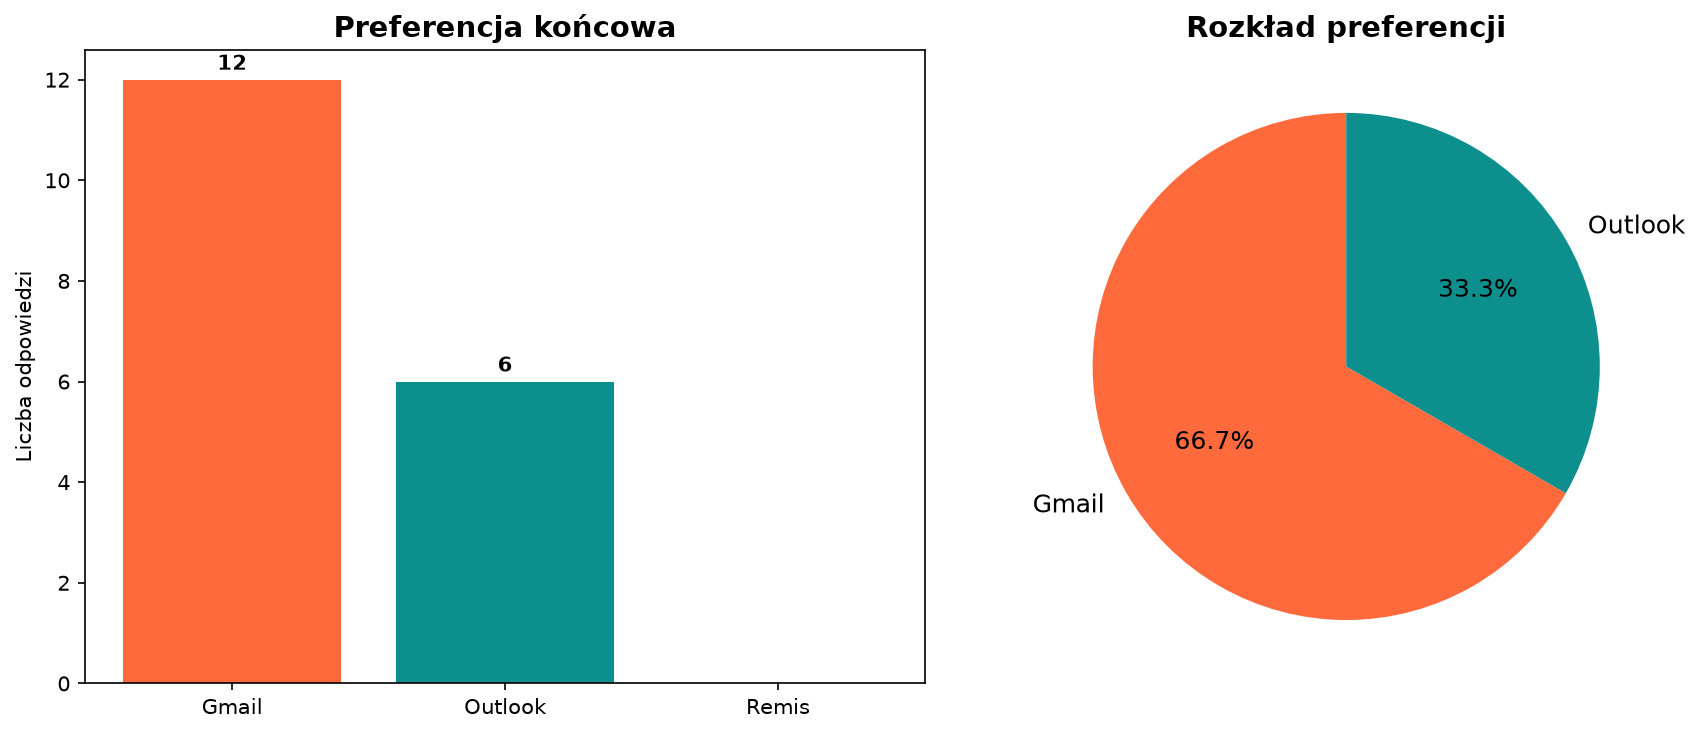
\includegraphics[width=0.75\textwidth]{charts/03_preference.png}
    \caption{Rozkład preferencji końcowej}
    \label{fig:preference}
\end{figure}

\subsection{Rozkład wieku respondentów}

Rysunek~\ref{fig:age_dist} przedstawia rozkład wiekowy uczestników badania. Zdecydowaną większość stanowią osoby w wieku 15--25 lat.

\begin{figure}[H]
    \centering
    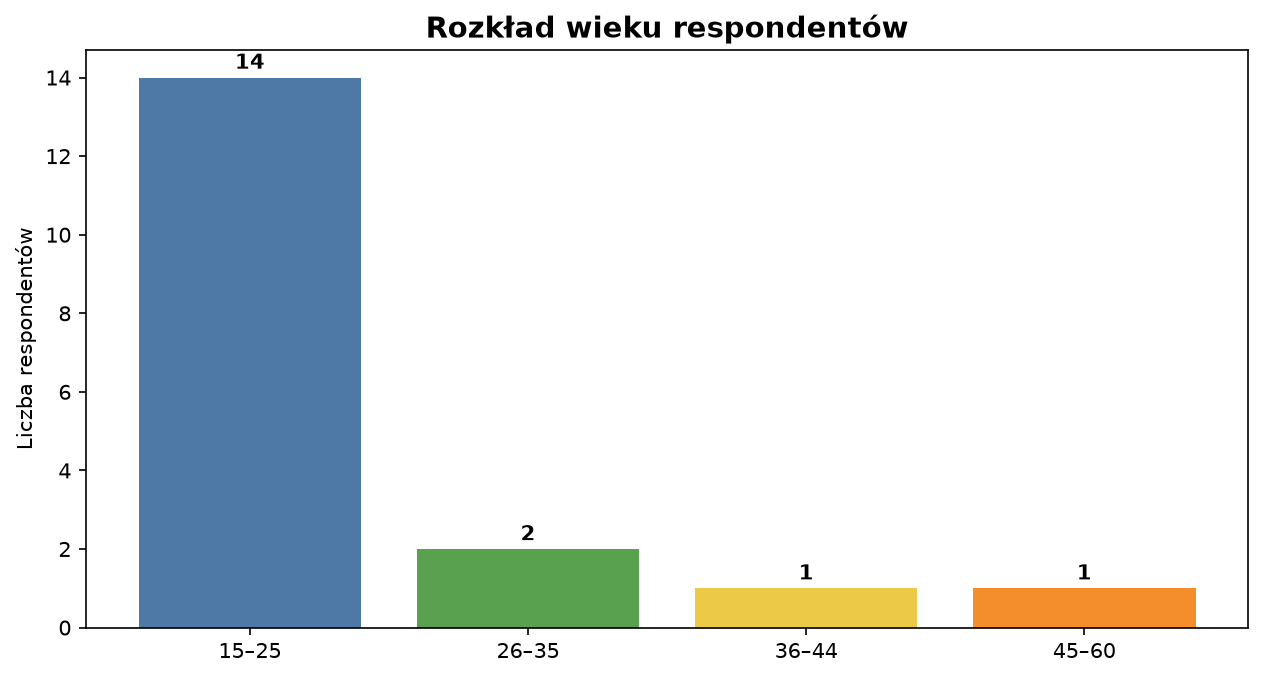
\includegraphics[width=0.75\textwidth]{charts/04_age_distribution.png}
    \caption{Histogram rozkładu wieku respondentów}
    \label{fig:age_dist}
\end{figure}

\subsection{Średnie ocen wg grup wiekowych}

Rysunek~\ref{fig:age_comp} porównuje średnie ocen Gmail i Outlook z podziałem na grupy wiekowe.

\begin{figure}[H]
    \centering
    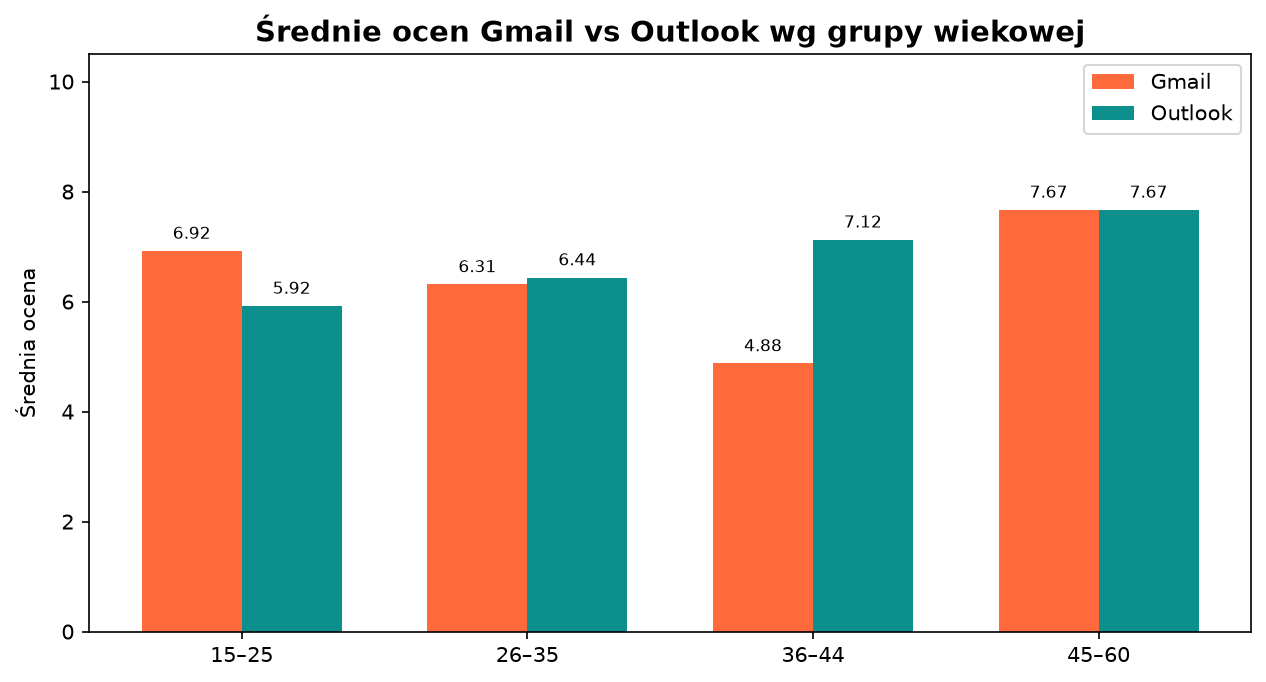
\includegraphics[width=0.75\textwidth]{charts/05_age_comparison.png}
    \caption{Średnie ocen Gmail vs Outlook wg grupy wiekowej}
    \label{fig:age_comp}
\end{figure}

\subsection{Preferencja wg grup wiekowych}

Rysunek~\ref{fig:age_pref} pokazuje rozkład preferencji końcowych z podziałem na grupy wiekowe.

\begin{figure}[H]
    \centering
    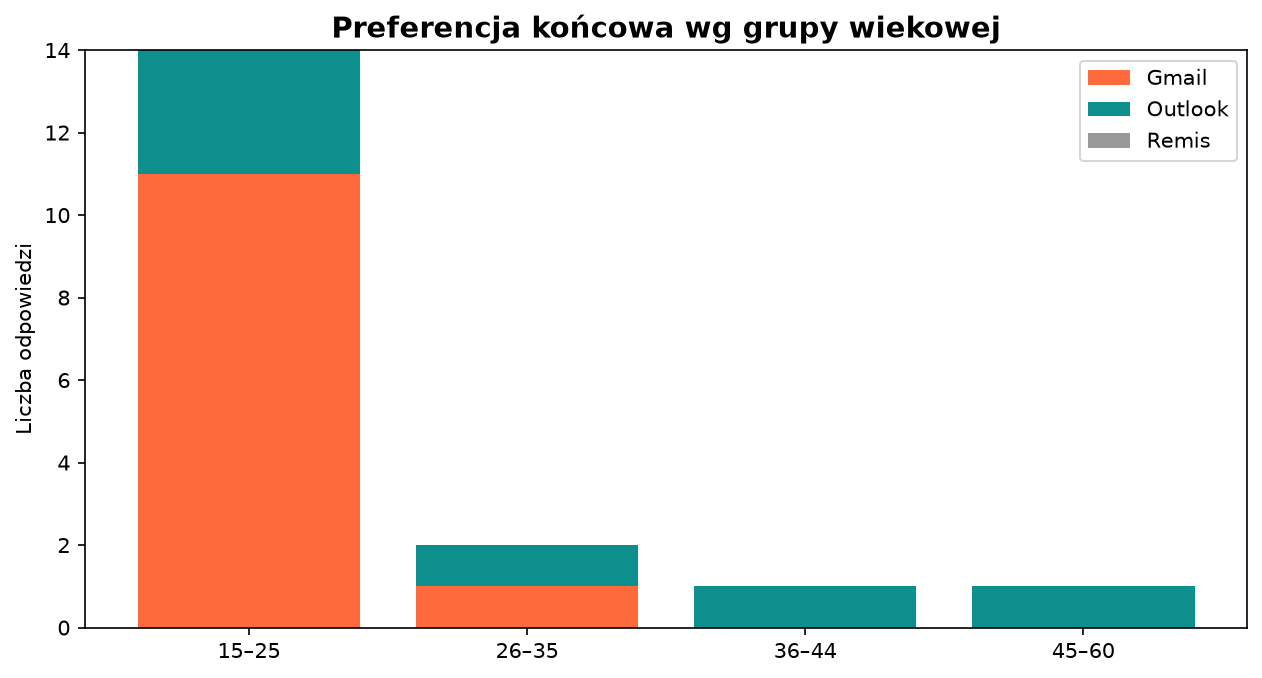
\includegraphics[width=0.75\textwidth]{charts/06_age_preference.png}
    \caption{Preferencja końcowa wg grupy wiekowej}
    \label{fig:age_pref}
\end{figure}

\subsection{Kompletność odpowiedzi}

Rysunek~\ref{fig:completeness} przedstawia rozkład kompletności odpowiedzi respondentów.

\begin{figure}[H]
    \centering
    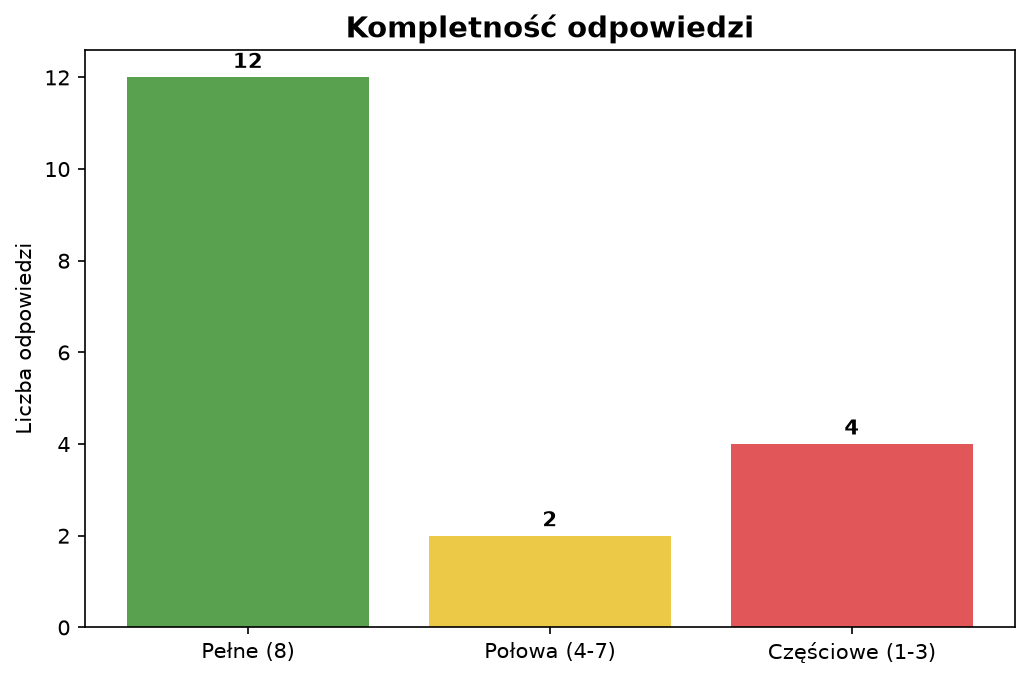
\includegraphics[width=0.6\textwidth]{charts/07_completeness.png}
    \caption{Kompletność odpowiedzi}
    \label{fig:completeness}
\end{figure}

%% === 6. WNIOSKI I PROPZYCJE MODYFIKACJI ===
\newpage
\section{Wnioski i propozycje modyfikacji/poprawek/ulepszeń}

\subsection{Wnioski ogólne}

\subsubsection{Dominacja Gmaila}

Gmail uzyskuje wyższe średnie oceny w \textbf{7 z 8 kryteriów}. Poniższa tabela przedstawia szczegółowe wyniki:

\begin{table}[H]
\centering
\caption{Porównanie średnich ocen Gmail vs Outlook}
\label{tab:porownanie}
\begin{tabularx}{\textwidth}{|X|c|c|X|}
\hline
\textbf{Kryterium} & \textbf{Gmail} & \textbf{Outlook} & \textbf{Przewaga} \\
\hline
Q1: Łatwość rozpoczęcia pracy & 7,00 & 6,06 & Gmail +0,94 \\
\hline
Q2: Czytelność nawigacji & 6,56 & 6,11 & Gmail +0,45 \\
\hline
Q3: Wyszukiwanie i filtrowanie & 6,76 & 5,59 & Gmail +1,17 \\
\hline
Q4: Tworzenie i edycja wiadomości & 6,57 & 6,71 & \textbf{Outlook +0,14} \\
\hline
Q5: Zarządzanie skrzynką & 6,17 & 5,92 & Gmail +0,25 \\
\hline
Q6: Widoczność statusu & 6,50 & 6,17 & Gmail +0,33 \\
\hline
Q7: Wydajność i szybkość & 6,75 & 6,17 & Gmail +0,58 \\
\hline
Q8: Ogólna satysfakcja & 7,33 & 6,42 & Gmail +0,91 \\
\hline
\end{tabularx}
\end{table}

\subsubsection{Rozkład preferencji końcowych}

\begin{itemize}[noitemsep]
    \item Gmail: 12 (66,7\%)
    \item Outlook: 6 (33,3\%)
    \item Remis: 0 (0,0\%)
\end{itemize}

Dwie trzecie respondentów wskazuje Gmail jako lepszą platformę. Żaden respondent nie wskazał remisu, co sugeruje wyraźne preferencje.

\subsubsection{Największe różnice}

\begin{enumerate}[noitemsep]
    \item \textbf{Wyszukiwanie (Q3):} Gmail +1,17 --- największa przewaga; respondenci doceniają precyzję i szybkość wyszukiwania Google
    \item \textbf{Łatwość rozpoczęcia (Q1):} Gmail +0,94 --- interfejs Gmail jest postrzegany jako bardziej intuicyjny
    \item \textbf{Ogólna satysfakcja (Q8):} Gmail +0,91 --- całościowe doświadczenie jest lepiej oceniane
\end{enumerate}

\subsubsection{Miejsca przewagi Outlooka}

\textbf{Tworzenie i edycja wiadomości (Q4):} Outlook +0,14 --- niewielka, ale jedyna przewaga. Może wynikać z bogatszego edytora formatowania (HTML, szablony) oraz integracji z pakietem Office.

\subsection{Wnioski z komentarzy respondentów}

Najczęściej pojawiające się motywy w wypowiedziach uczestników:

\begin{table}[H]
\centering
\caption{Analiza komentarzy respondentów}
\label{tab:komentarze}
\begin{tabularx}{\textwidth}{|X|c|X|}
\hline
\textbf{Motyw} & \textbf{Liczba wzmianek} & \textbf{Przykładowe wypowiedzi} \\
\hline
Gmail intuicyjny/prosty & 5 & ``Gmail jest bardziej intuicyjny'', ``Gmail wygrywa prostotą'' \\
\hline
Outlook do pracy biurowej & 4 & ``Outlook lepszy do pracy biurowej'' \\
\hline
Outlook wolny & 1 & ``Outlook męczy mnie wolnym działaniem'' \\
\hline
Gmail lepsze wyszukiwanie & 1 & ``Gmail ma lepsze wyszukiwanie'' \\
\hline
Brak dużej różnicy & 1 & ``Po dłuższym użytkowaniu nie widzę dużej różnicy'' \\
\hline
\end{tabularx}
\end{table}

\textbf{Kluczowy wniosek:} Gmail jest postrzegany jako prostszy i bardziej intuicyjny, podczas gdy Outlook jest kojarzony z pracą biurową (kalendarz, integracja z Office).

\subsection{Rekomendacje dla Gmail}

Na podstawie danych, w których Outlook przewyższa Gmail:

\begin{enumerate}
    \item \textbf{Edycja wiadomości (Q4):} Outlook ma lepszy edytor --- Gmail powinien rozważyć:
    \begin{itemize}[noitemsep]
        \item Dodanie zaawansowanego formatowania HTML
        \item Wprowadzenie szablonów wiadomości
        \item Lepszą integrację z edytorami tekstu
    \end{itemize}

    \item \textbf{Zarządzanie skrzynką (Q5):} Przewaga Gmaila jest niewielka (+0,25) --- warto:
    \begin{itemize}[noitemsep]
        \item Ulepszyć masowe operacje (oznaczanie, przenoszenie)
        \item Dodać inteligentne foldery/widoki
    \end{itemize}
\end{enumerate}

\subsection{Rekomendacje dla Outlooka}

Outlook przegrywa w 7 z 8 kryteriów --- priorytowe obszary ulepszeń:

\begin{enumerate}
    \item \textbf{Wyszukiwanie (Q3):} Outlook przegrywa najbardziej (5,59 vs 6,76)
    \begin{itemize}[noitemsep]
        \item Wdrożenie pełnotekstowego wyszukiwania z operatorami logicznymi
        \item Lepsze filtrowanie i sortowanie wyników
    \end{itemize}

    \item \textbf{Łatwość rozpoczęcia pracy (Q1):} Interfejs jest mniej intuicyjny
    \begin{itemize}[noitemsep]
        \item Uproszczenie domyślnego widoku
        \item Redukcja liczby elementów na ekranie
        \item Lepszy onboarding dla nowych użytkowników
    \end{itemize}

    \item \textbf{Wydajność (Q7):} Outlook jest postrzegany jako wolniejszy
    \begin{itemize}[noitemsep]
        \item Optymalizacja ładowania interfejsu
        \item Redukcja opóźnień przy przełączaniu między widokami
        \item Caching częściej używanych danych
    \end{itemize}

    \item \textbf{Ogólna satysfakcja (Q8):} Niska ocena (6,42) wynika z kumulacji problemów
    \begin{itemize}[noitemsep]
        \item Kompleksowy redesign interfejsu z naciskiem na prostotę
    \end{itemize}
\end{enumerate}

\subsection{Propozycje dalszych badań}

\begin{enumerate}
    \item \textbf{Badanie z podziałem na grupy zaawansowania} --- obecnie poziom doświadczenia nie jest zbierany w formularzu; warto dodać pole (początkujący/średniozaawansowany/zaawansowany) i analizować wyniki wg doświadczenia

    \item \textbf{Pomiary czasu wykonania zadań} --- uzupełnienie ocen subiektywnych o obiektywne pomiary czasu (np. ``ile czasu zajęło znalezienie wiadomości X?'')

    \item \textbf{Testy A/B konkretnych zmian} --- po identyfikacji słabych punktów, testowanie konkretnych modyfikacji interfejsu na reprezentatywnej grupie

    \item \textbf{Większa próba} --- zwiększenie liczby respondentów do min. 30--50 osób w celu uzyskania bardziej miarodajnych statystyk, zwłaszcza w grupach 26--35, 36--44 i 45--60

    \item \textbf{Badanie longitudinalne} --- śledzenie zmian ocen w czasie (przed i po redesignie interfejsu)
\end{enumerate}

\end{document}
